% Created 2014-03-26 Wed 18:41
\documentclass[presentation,smaller]{beamer}
\usepackage[utf8]{inputenc}
\usepackage[T1]{fontenc}
\usepackage{fixltx2e}
\usepackage{graphicx}
\usepackage{longtable}
\usepackage{float}
\usepackage{wrapfig}
\usepackage{rotating}
\usepackage[normalem]{ulem}
\usepackage{amsmath}
\usepackage{textcomp}
\usepackage{marvosym}
\usepackage{wasysym}
\usepackage{amssymb}
\usepackage{hyperref}
\tolerance=1000
\usepackage{color}
\usepackage{listings}
\usepackage[utf8]{inputenc}
\usepackage{hyperref}
\hypersetup{
colorlinks,%
citecolor=black,%
filecolor=black,%
linkcolor=blue,%
urlcolor=black
}
\institute{Affilations:  Academia Sinica, o0o.nu, chroot.org}
\setbeamersize{text margin left=0.2cm}
\usetheme{Szeged}
\author{Vladimir Kropotov, Vitaly Chetvertakov, Fyodor Yarochkin\\\ RusCrypto 2014}
\date{March 25-28, 2014}
\title{Incident Response tactics with Compromise Indicators}
\hypersetup{
  pdfkeywords={},
  pdfsubject={},
  pdfcreator={Emacs 24.3.50.1 (Org mode 8.2.5c)}}
\begin{document}

\maketitle
\begin{frame}{Outline}
\tableofcontents
\end{frame}



\section{Basics}
\label{sec-1}
\begin{frame}[label=sec-1-1]{Introduction}
\alert{Indicators of Compromise}

Indicator of compromise (IOC) in computer forensics is an artifact
observed on network or in operating system that with high confidence
indicates a computer intrusion.

\url{http://en.wikipedia.org/wiki/Indicator_of_compromise}
\end{frame}


\begin{frame}[label=sec-1-2]{IOC workflow}
A typical flow with Indicators of Compromise:
\tiny
source: Sophisticated indicators for the modern threat landscape, 2012
paper
\normalsize
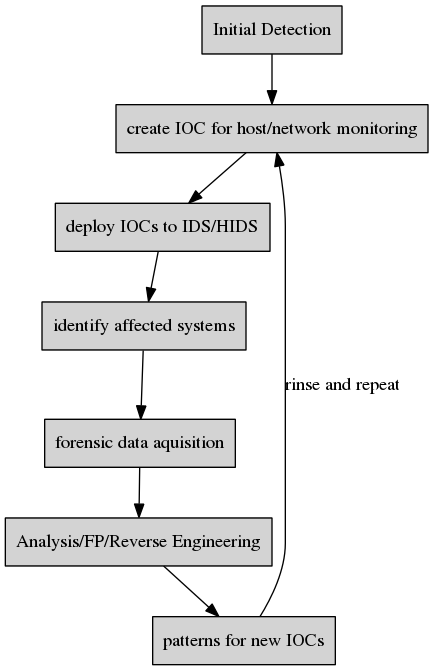
\includegraphics[width=8cm]{images/ioc.png}
\end{frame}
\section{Standards}
\label{sec-2}
\begin{frame}[label=sec-2-1]{Standards: OpenIOC}
OpenIOC - Mandiant-backed effort for unform representation of IOC
(now FireEye)
\url{http://www.openioc.org/}
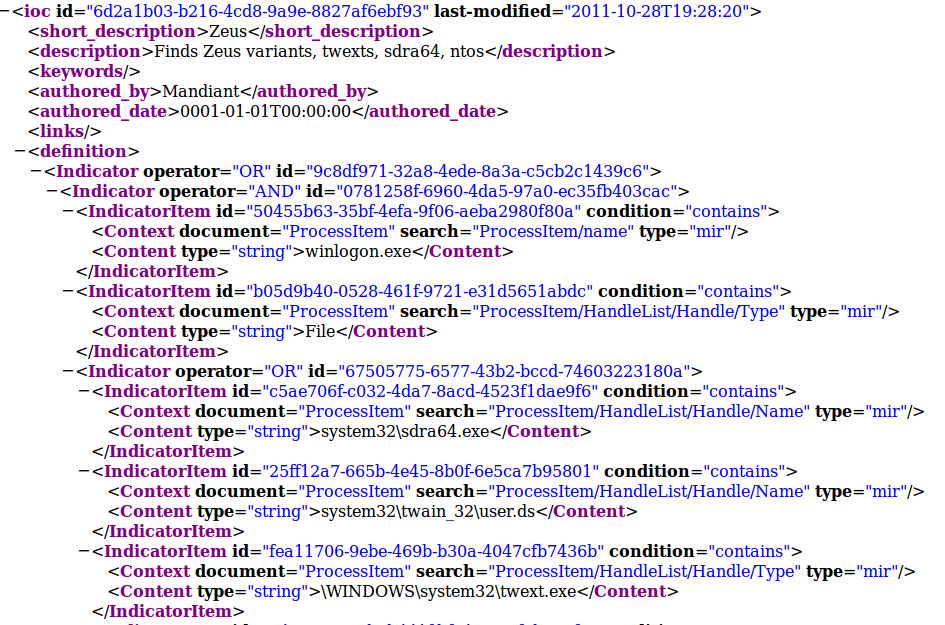
\includegraphics[width=.9\linewidth]{images/zeus-ioc.png}
\end{frame}
\begin{frame}[label=sec-2-2]{Standards: Mitre}
Mitre CybOX:
\url{http://cybox.mitre.org/}
\url{https://github.com/CybOXProject/Tools}
\url{https://github.com/CybOXProject/openioc-to-cybox}
Mitre CAPEC:
\url{http://capec.mitre.org/}
Mitre STIX:
\url{http://stix.mitre.org/}
Mitre TAXII
\url{http://taxii.mitre.org/}
\end{frame}
\section{Tools}
\label{sec-3}

\begin{frame}[label=sec-3-1]{Open-source tools}
OpenIOC manipulation
\url{https://github.com/STIXProject/openioc-to-stix}
\url{https://github.com/tklane/openiocscripts} 

Mantis Threat Intelligence Framework
 \url{https://github.com/siemens/django-mantis.git}
Mantis supports STIX/CybOX/IODEF/OpenIOC etc via
importers: \url{https://github.com/siemens/django-mantis-openioc-importer}


Search splunk data for IOC indicators:
\url{https://github.com/technoskald/splunk-search}

Our framework:
\url{http://github.com/fygrave/iocmap/}
\end{frame}
\section{Sharing IOCs}
\label{sec-4}
\begin{frame}[label=sec-4-1]{Online Sharing of IOCs}
\url{http://iocbucket.com/}

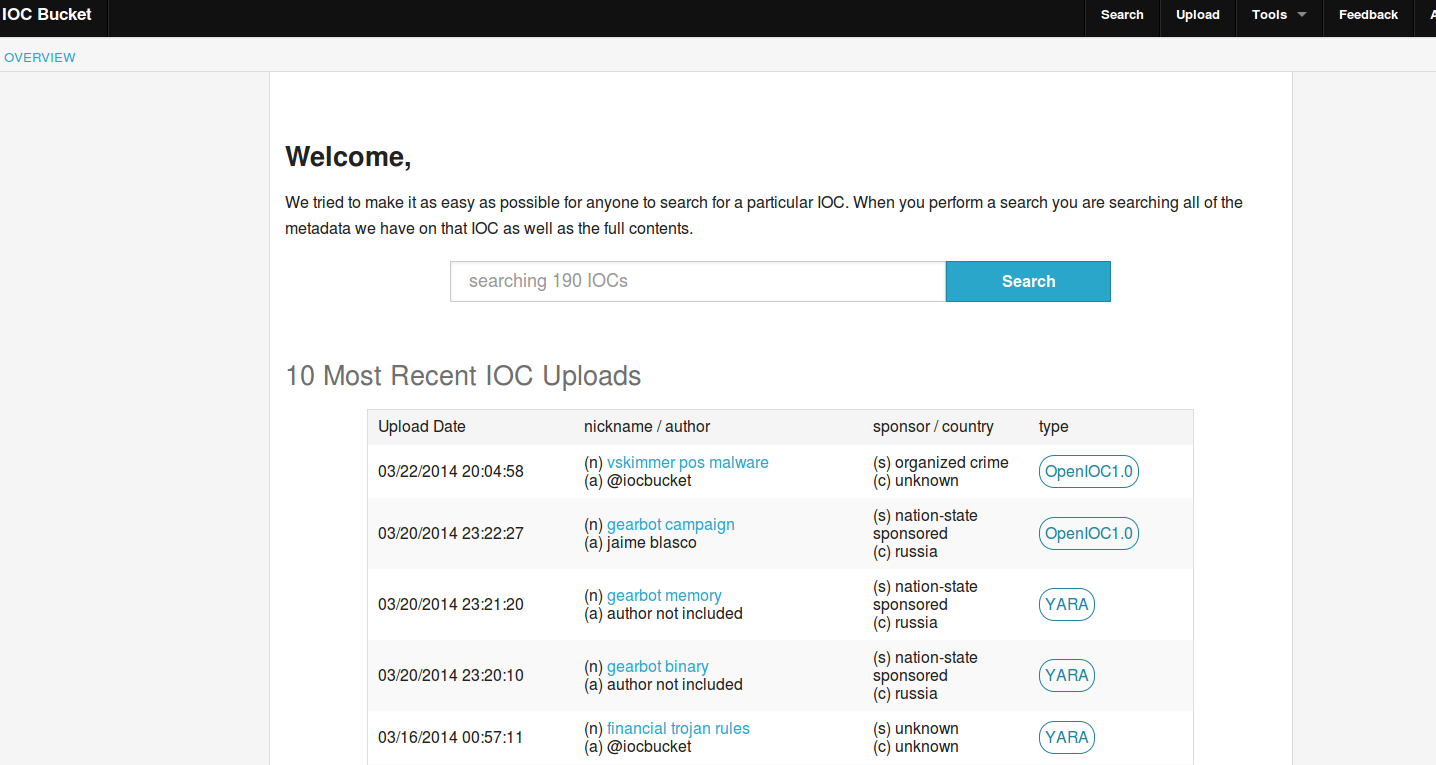
\includegraphics[width=.9\linewidth]{images/iocbucket.png}
\end{frame}
\begin{frame}[label=sec-4-2]{Policies on Sharing}
Policies on sharing IOCs:

\begin{itemize}
\item what to be shared/can be shared
\item who to share with
\item when to share
\end{itemize}
\end{frame}
\section{IOCs composites}
\label{sec-5}
\begin{frame}[label=sec-5-1]{Where to look for IOCs:}
\begin{itemize}
\item Outbound Network Traffic
\item User Activities/Failed Logins
\item User profile folders
\item Administrative Access
\item Access from unsual IP addresses
\item Database IO: excessive READs
\item Size of responses of web pages
\item Unusual access to particular files within Web Application (backdoor)
\item Unusual port/protocol connections
\item DNS and HTTP traffic requests
\item Suspicious Scripts, Executables and Data Files
\end{itemize}
\end{frame}
\begin{frame}[label=sec-5-2]{Challenges}
Why we need IOCs? because it makes it easier to
systematically describe knowledge about breaches.

\begin{itemize}
\item Identifying intrusions is hard
\item Unfair game:
\begin{itemize}
\item defender should protect all the assets
\item attacker only needs to 'poop' one system.
\end{itemize}
\item Identifying targeted, organized intrusions is even harder
\item Minor anomalous events are important when put together
\item Seeing global picture is a mast
\item Details matter
\item Attribution is hard
\end{itemize}
\end{frame}
\begin{frame}[label=sec-5-3]{Challenges}
\alert{All networks are compromised}


The difference between a good security team and a bad security team is
that with a bad security team you will never know that you've been
compromised.
\end{frame}
\section{Case Study}
\label{sec-6}
\begin{frame}[label=sec-6-1]{An Example}
A Network compromise case study:
\begin{itemize}
\item Attackers broke via a web vuln.
\item Attackers gained local admin access
\item Attackers created a local user
\item Attackers started probing other machines for default user ids
\item Attackers launched tunneling tools – connecting back to C2
\item Attackers installed RATs to maintain access
\end{itemize}
\end{frame}
\begin{frame}[label=sec-6-2]{Indicators}
So what are the compromise indicators here?

\begin{itemize}
\item Where did attackers come from? (IP)
\item What vulnerability was exploited? (pattern)
\item What web backdoor was used? (pattern, hash)
\item What tools were uploaded? (hashes)
\item What users were created locally? (username)
\item What usernames were probed on other machines
\end{itemize}
\end{frame}

\begin{frame}[fragile,label=sec-6-3]{Good or Bad?}
 \tiny
\lstset{language=sh,numbers=none}
\begin{lstlisting}
File Name                       : RasTls.exe
File Size                       : 105 kB
File Modification Date/Time     : 2009:02:09 19:42:05+08:00
File Type                       : Win32 EXE
MIME Type                       : application/octet-stream
Machine Type                    : Intel 386 or later, and compatibles
Time Stamp                      : 2009:02:02 13:38:37+08:00
PE Type                         : PE32
Linker Version                  : 8.0
Code Size                       : 49152
Initialized Data Size           : 57344
Uninitialized Data Size         : 0
Entry Point                     : 0x3d76
OS Version                      : 4.0
Image Version                   : 0.0
Subsystem Version               : 4.0
Subsystem                       : Windows GUI
File Version Number             : 11.0.4010.7
Product Version Number          : 11.0.4010.7
File OS                         : Windows NT 32-bit
Object File Type                : Executable application
Language Code                   : English (U.S.)
Character Set                   : Windows, Latin1
Company Name                    : Symantec Corporation
File Description                : Symantec 802.1x Supplicant
File Version                    : 11.0.4010.7
Internal Name                   : dot1xtray
\end{lstlisting}
\normalsize
\end{frame}
\begin{frame}[fragile,label=sec-6-4]{It really depends on context}
 \lstset{language=sh,numbers=none}
\begin{lstlisting}
RasTls.DLL 
RasTls.DLL.msc
RasTls.exe
\end{lstlisting}

\url{http://msdn.microsoft.com/en-us/library/ms682586(v=VS.85).aspx}

\alert{Dynamic-Link Library Search Order}


\includegraphics[width=3cm]{images/pantsdown.jpg}
\end{frame}


\section{More on Tools}
\label{sec-7}
\begin{frame}[label=sec-7-1]{Tools for Dynamic Detection of IOC}
\begin{itemize}
\item Snort
\item Yara + yara-enabled tools
\item Moloch
\item Splunk/Log search
\end{itemize}
\end{frame}
\begin{frame}[fragile,label=sec-7-2]{Tools for Dynamic Detection}
 \begin{itemize}
\item Moloch
\begin{itemize}
\item Moloch supports Yara (IOCs can be directly applied)
\item Moloch has tagger plugin:
\end{itemize}
\end{itemize}
\lstset{language=sh,numbers=none}
\begin{lstlisting}
# tagger.so
# provides ability to import text files with IP and/or hostnames 
# into a sensor that would cause autotagging of all matching sessions
plugins=tagger.so
taggerIpFiles=blacklist,tag,tag,tag...
taggerDomainFiles=domainbasedblacklists, tag, tag, tag
\end{lstlisting}
\end{frame}
\begin{frame}[label=sec-7-3]{Sources of IOCs}
\begin{itemize}
\item ioc bucket:
\end{itemize}
\url{http://iocbucket.com}

\begin{itemize}
\item Public blacklists/trackers could also be used as source:
\end{itemize}

\url{https://zeustracker.abuse.ch/blocklist.php?download=ipblocklist}

\url{https://zeustracker.abuse.ch/blocklist.php?download=domainblocklist}

\begin{itemize}
\item Eset IOC repository
\end{itemize}
\url{https://github.com/eset/malware-ioc}

more coming?
\end{frame}
\begin{frame}[fragile,label=sec-7-4]{where to mine IOC}
 \begin{itemize}
\item passive HTTP (keep your data recorded)
\item passive DNS
\end{itemize}

These platforms provide
ability to mine traffic or patterns from the past
based on IOC similarity

\alert{show me all the packets similar to this IOC}

We implemented a whois service for IOC look-ups
\lstset{language=sh,numbers=none}
\begin{lstlisting}
whois -h ioc.host.com   attribute:value+attribute:value
\end{lstlisting}
\end{frame}

\begin{frame}[label=sec-7-5]{Mining IOCs from your own data}
\begin{itemize}
\item find and investigate incident
\item Or even read paper
\item determine indicators and test it in YOUR Environment
\item use new indicators in the future

\alert{see IOC cycle we mentioned earlier}
\end{itemize}
\end{frame}
\begin{frame}[fragile,label=sec-7-6]{Example}
 If event chain leads to compromise
\tiny
\lstset{language=sh,numbers=none}
\begin{lstlisting}
http:// liapolasens[.]info/indexm.html

http:// liapolasens[.]info/counter.php?t=f&v=win%2011,7,700,169&a=true

http:// liapolasens[.]info/354RIcx

http:// liapolasens[.]info/054RIcx
\end{lstlisting}
\normalsize
What to do?
\end{frame}
\begin{frame}[fragile,label=sec-7-7]{Use YARA, or tune your own tools}
 \tiny
\lstset{language=sh,numbers=none}
\begin{lstlisting}
rule susp_params_in_url_kind_of_fileless_bot_drive_by
{
        meta:
        date = "oct 2013"
        description = "Landing hxxp://jdatastorelame.info/indexm.html  04.10.2013 13:14  108.62.112.84  "  
        description1 =  " Java Sploit hxxp://jdatastorelame.info/054RIwj     "


    strings:
        $string0 = "http"
        $string1 = "indexm.html"
        $string2 = "054RI"



    condition:
        all of them
}
\end{lstlisting}
\normalsize
\end{frame}
\begin{frame}[fragile,label=sec-7-8]{Use snort to catch suspicious traffic:}
 \tiny
\lstset{language=sh,numbers=none}
\begin{lstlisting}
# many plugX deployments connect to google DNS when not in use
alert tcp !$DNS_SERVERS any -> 8.8.8.8 53 (msg:"APT possible PlugX Google DNS TCP
port 53 connection attempt"; classtype:misc-activity; sid:500000112;
rev:1;)
\end{lstlisting}
\normalsize
\end{frame}

\begin{frame}[label=sec-7-9]{GRR: Google Rapid Response:}
\url{http://code.google.com/p/grr/}

Hunting IOC artifacts with GRR

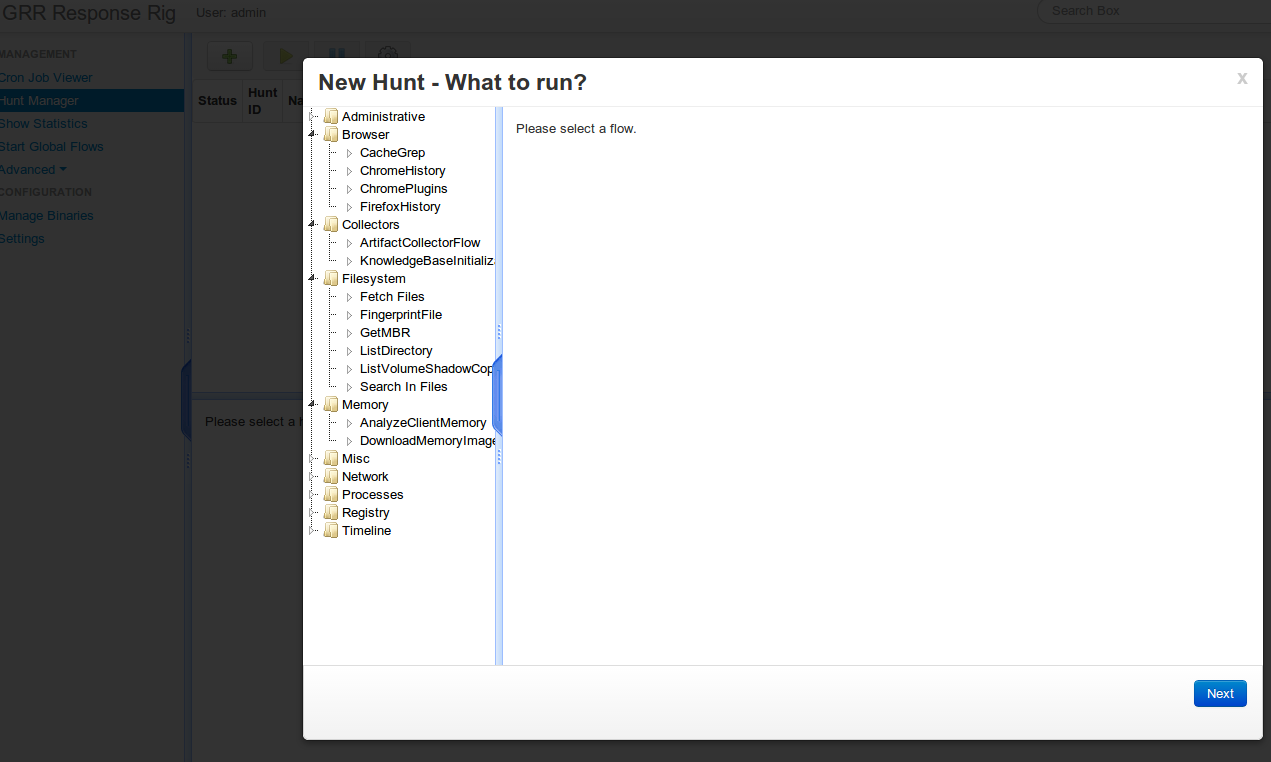
\includegraphics[width=.9\linewidth]{images/grr.png}
\end{frame}
\begin{frame}[label=sec-7-10]{GRR: Creating rules}
\begin{columns}
\begin{column}{0.5\textwidth}
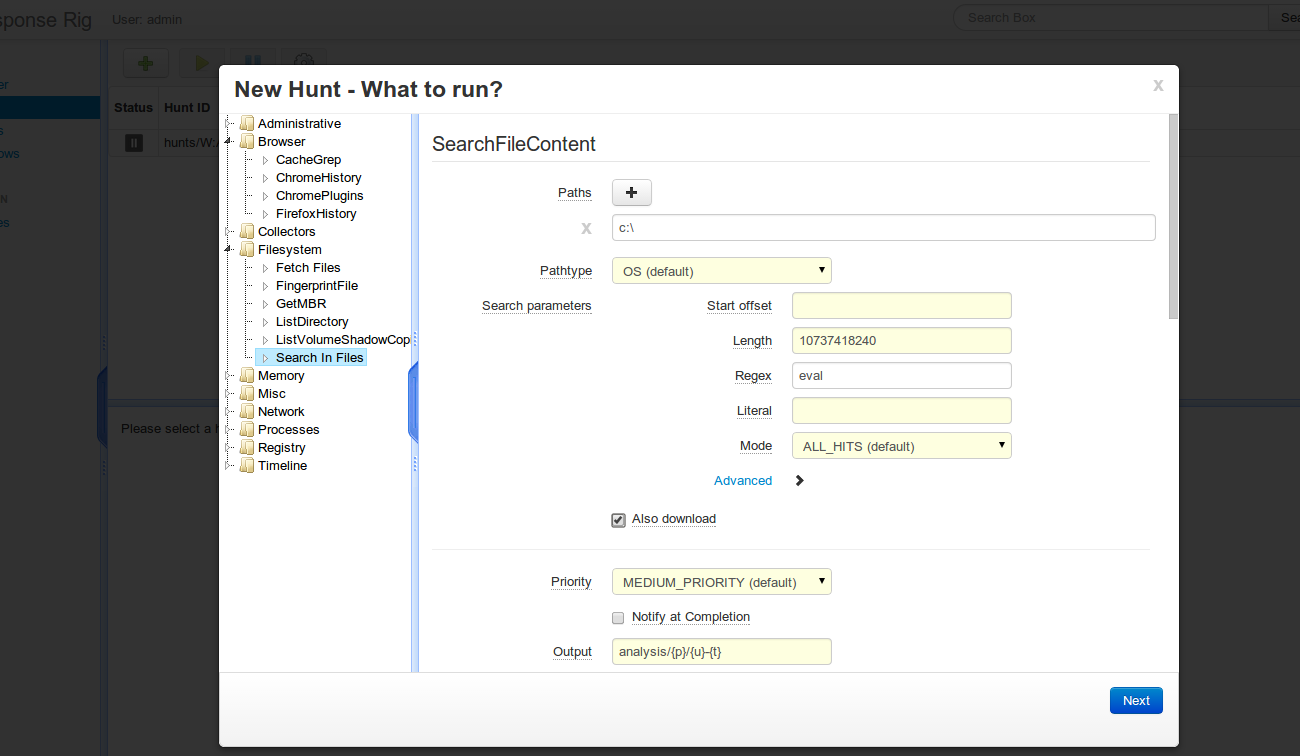
\includegraphics[width=.9\linewidth]{images/grr03.png}
\end{column}

\begin{column}{0.5\textwidth}
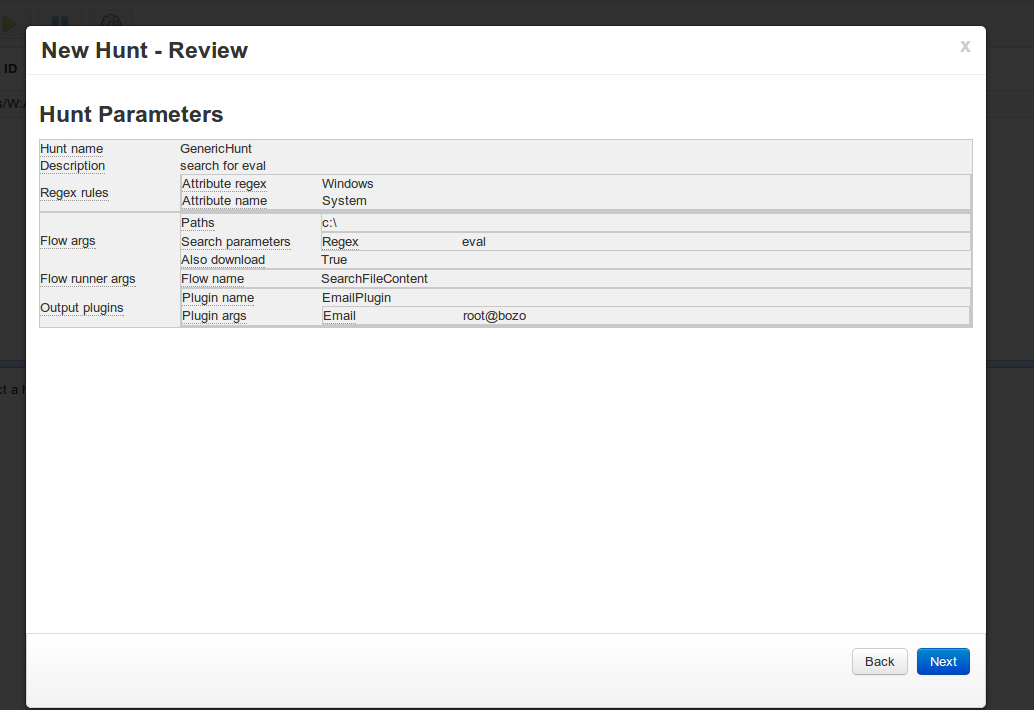
\includegraphics[width=.9\linewidth]{images/grr04.png}
\end{column}
\end{columns}
\end{frame}
\begin{frame}[label=sec-7-11]{GRR: hunt in progress}
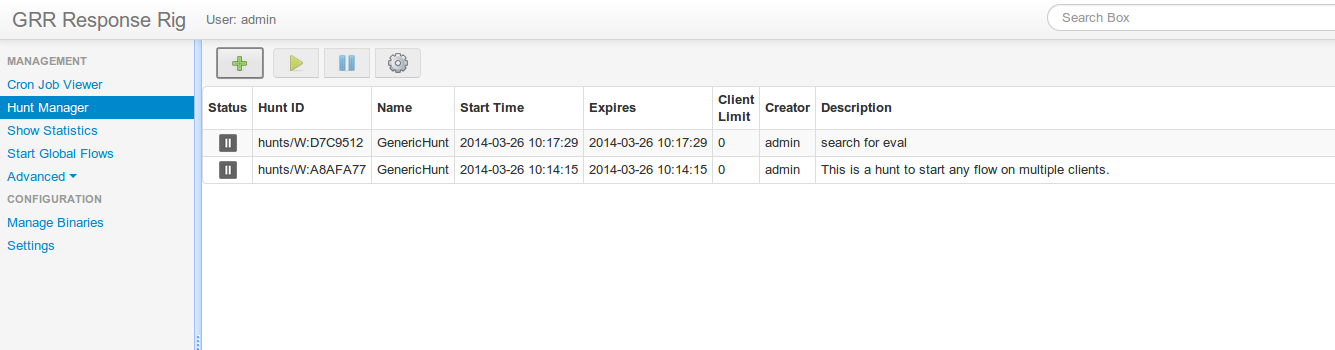
\includegraphics[width=.9\linewidth]{images/grr05.png}
\end{frame}
\begin{frame}[label=sec-7-12]{IOC management portal}
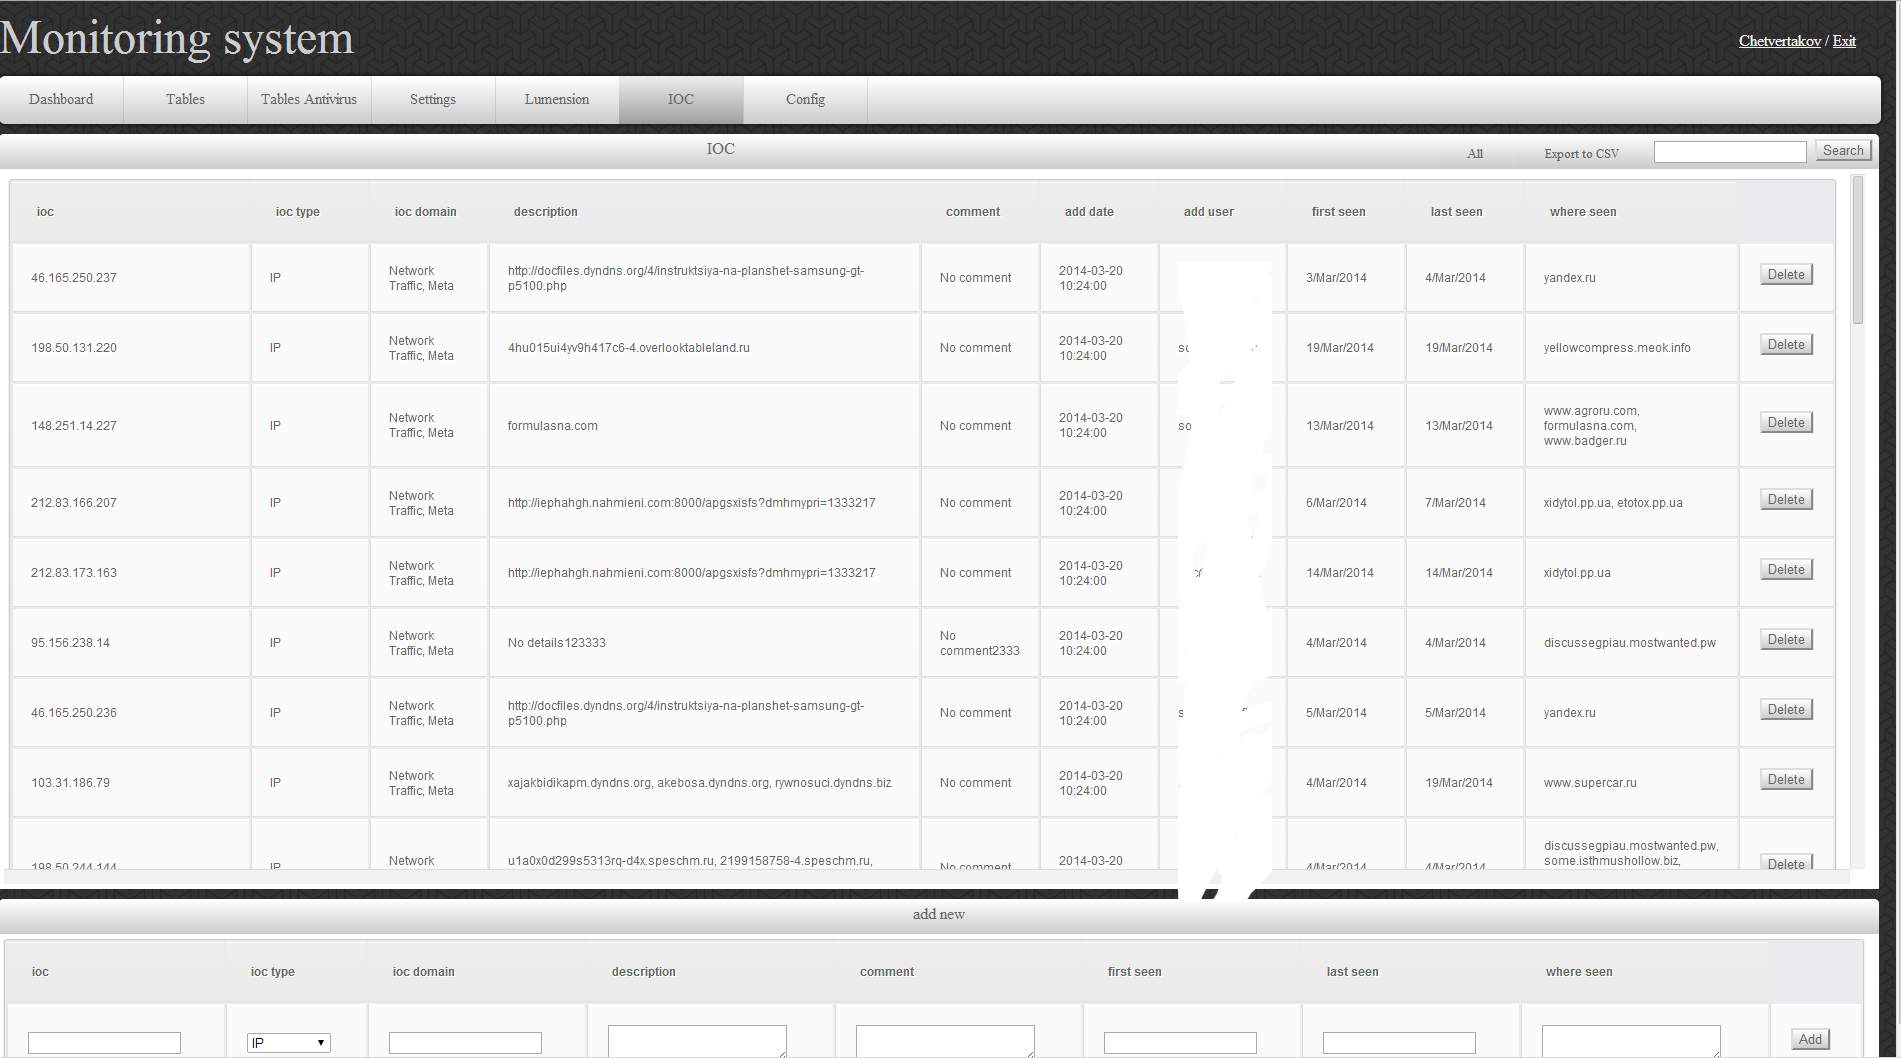
\includegraphics[width=14cm]{images/ioc01.png}
\end{frame}

\begin{frame}[fragile,label=sec-7-13]{IOC exportable to json}
 \tiny
\lstset{language=C,numbers=none}
\begin{lstlisting}
{ "8000" : { "IP" : ['212.83.167.192', '212.83.170.14', '212.83.170.22', '212.83.173.163', '212.83.166.207'] },
"fyflash" : { "IP" : ['103.246.246.103', '74.126.177.68', '204.200.222.136', '194.183.224.75', 
'76.73.80.188', '74.126.177.70', '192.74.246.219', '74.126.177.241'] , 
"Domain" : ['wmi.ns01.us ', 'proxy.ddns.info ', 'windows.ddns.us ', 
'microsafes.no-ip.org ', 'fuckchina.govnb.com ', 'ids.ns01.us ', 
'updatedns.ns01.us ', 'updatedns.ns02.us ', 
'adservice.no-ip.org ', 'java.ns1.name '] , 
"MD5" : ['7d810e3564c4eb95bcb3d11ce191208e', '1ec5141051776ec9092db92050192758'] },
"btc" : { "IP" : ['184.106.146.244'] },
"slvbuso" : { "MD5" : ['45645F17E3B014B9BCE89A793F5775B2'] , "Domain" : ['helldark.biz'] },
"sp" : { "IP" : ['194.58.91.186', '95.156.238.14', '192.95.46.0', '198.50.131.220', '198.50.244.144',
 '198.50.140.72', '95.156.238.5', '192.95.46.25'] },
"pw" : { "IP" : ['185.8.106.97', '195.2.253.25'] },
"sophMdropFQI" : { "MD5" : ['cf656fd9f839a5cd56bb999197745a49'] , "Domain" : ['samiollo.org'] },
"symsr" : { "IP" : ['212.95.32.52', '95.211.130.132', '123.45.67.89'] ,
 "Domain" : ['wertdghbyrukl.ch', 'rgtryhbgddtyh.biz'] } 
"fakeinstr" : { "IP" : ['46.165.250.237', '46.165.250.236', '46.165.250.197'] },
"msProlaco" : { "Domain" : ['kathell.com', 'coginix.org'] } }
\end{lstlisting}
\normalsize
\end{frame}

\begin{frame}[label=sec-7-14]{and every manager loves graphs :p}
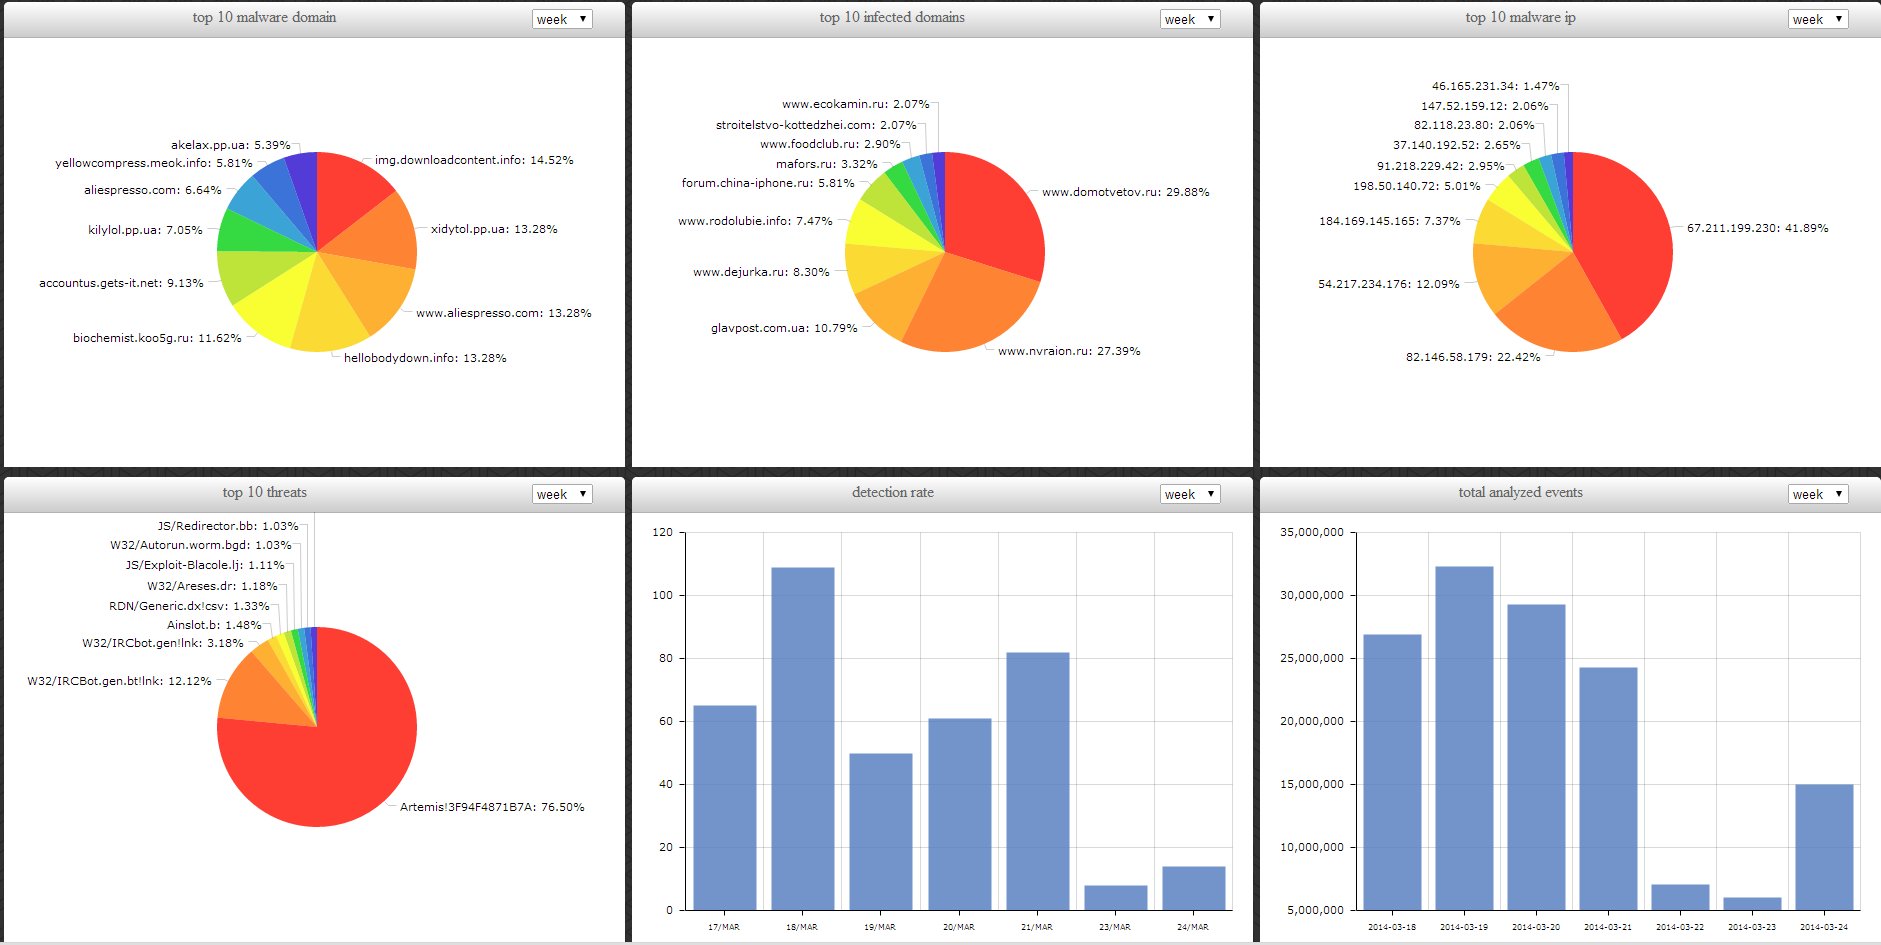
\includegraphics[width=14cm]{images/ioc02.png}
\end{frame}

\section{Questions}
\label{sec-8}
\begin{frame}[label=sec-8-1]{Q and A}
Or contact us at \ldots{}
\end{frame}
% Emacs 24.3.50.1 (Org mode 8.2.5c)
\end{document}